%\documentclass[handout]{beamer}
%\documentclass[handout,10pt,slidestop,mathserif]{beamer}
%\usepackage{pgfpages}
%\pgfpagesuselayout{2 on 1}
\documentclass[10pt,slidestop,mathserif]{beamer}
\usetheme{Madrid}
\usecolortheme{seahorse}

\usepackage{tabularx}
\usepackage{verbatim}
\usepackage{graphics}
\usepackage{graphicx}
\usepackage{Sweave}
\usepackage{moreverb}
\usepackage{pgf}
\usepackage{tikz}
\usepackage[notocbib]{apacite}

\newcommand{\putat}[3]{\begin{picture}(0,0)(0,0)\put(#1,#2){#3}\end{picture}}
  
\newenvironment{changemargin}[2]{%
  \begin{list}{}{%
    \setlength{\topsep}{0pt}%
    \setlength{\leftmargin}{#1}%
    \setlength{\rightmargin}{#2}%
    \setlength{\listparindent}{\parindent}%
    \setlength{\itemindent}{\parindent}%
    \setlength{\parsep}{\parskip}%
  }%
  \item[]}{\end{list}}

%% Define a new 'leo' style for the package that will use a smaller font.
\makeatletter
\def\url@leostyle{%
  \@ifundefined{selectfont}{\def\UrlFont{\sf}}{\def\UrlFont{\tiny\ttfamily}}}
\makeatother

\title[Dissertation Proposal]{A National Study Comparing Charter and Traditional Public Schools Using Propensity Score Analysis}
\subtitle{Dissertation Proposal}
\author[Bryer]{Jason M. Bryer}
\institute[University at Albany]{Division of Educational Psychology \& Methodology\\University at Albany}
\date{December 19, 2011}

\begin{document}


\frame{\titlepage}
\frame{\frametitle{Agenda}\tableofcontents[hideallsubsections]}

\section{Overview}

\begin{frame}
	\frametitle{What are Charter Schools?}
	The first charter school opened in Minnesota in 1991
	In principle, charter schools have opted out of bureaucratic rules and union contracts in order to gain academic autonomy. The standard argument has become that this autonomy will lead to higher student test scores and better academic environments \cite{Wells2002}. The idea is that, under the charter framework, teachers, administrators, students and the community that comprise the charter school would be free to innovate
	
	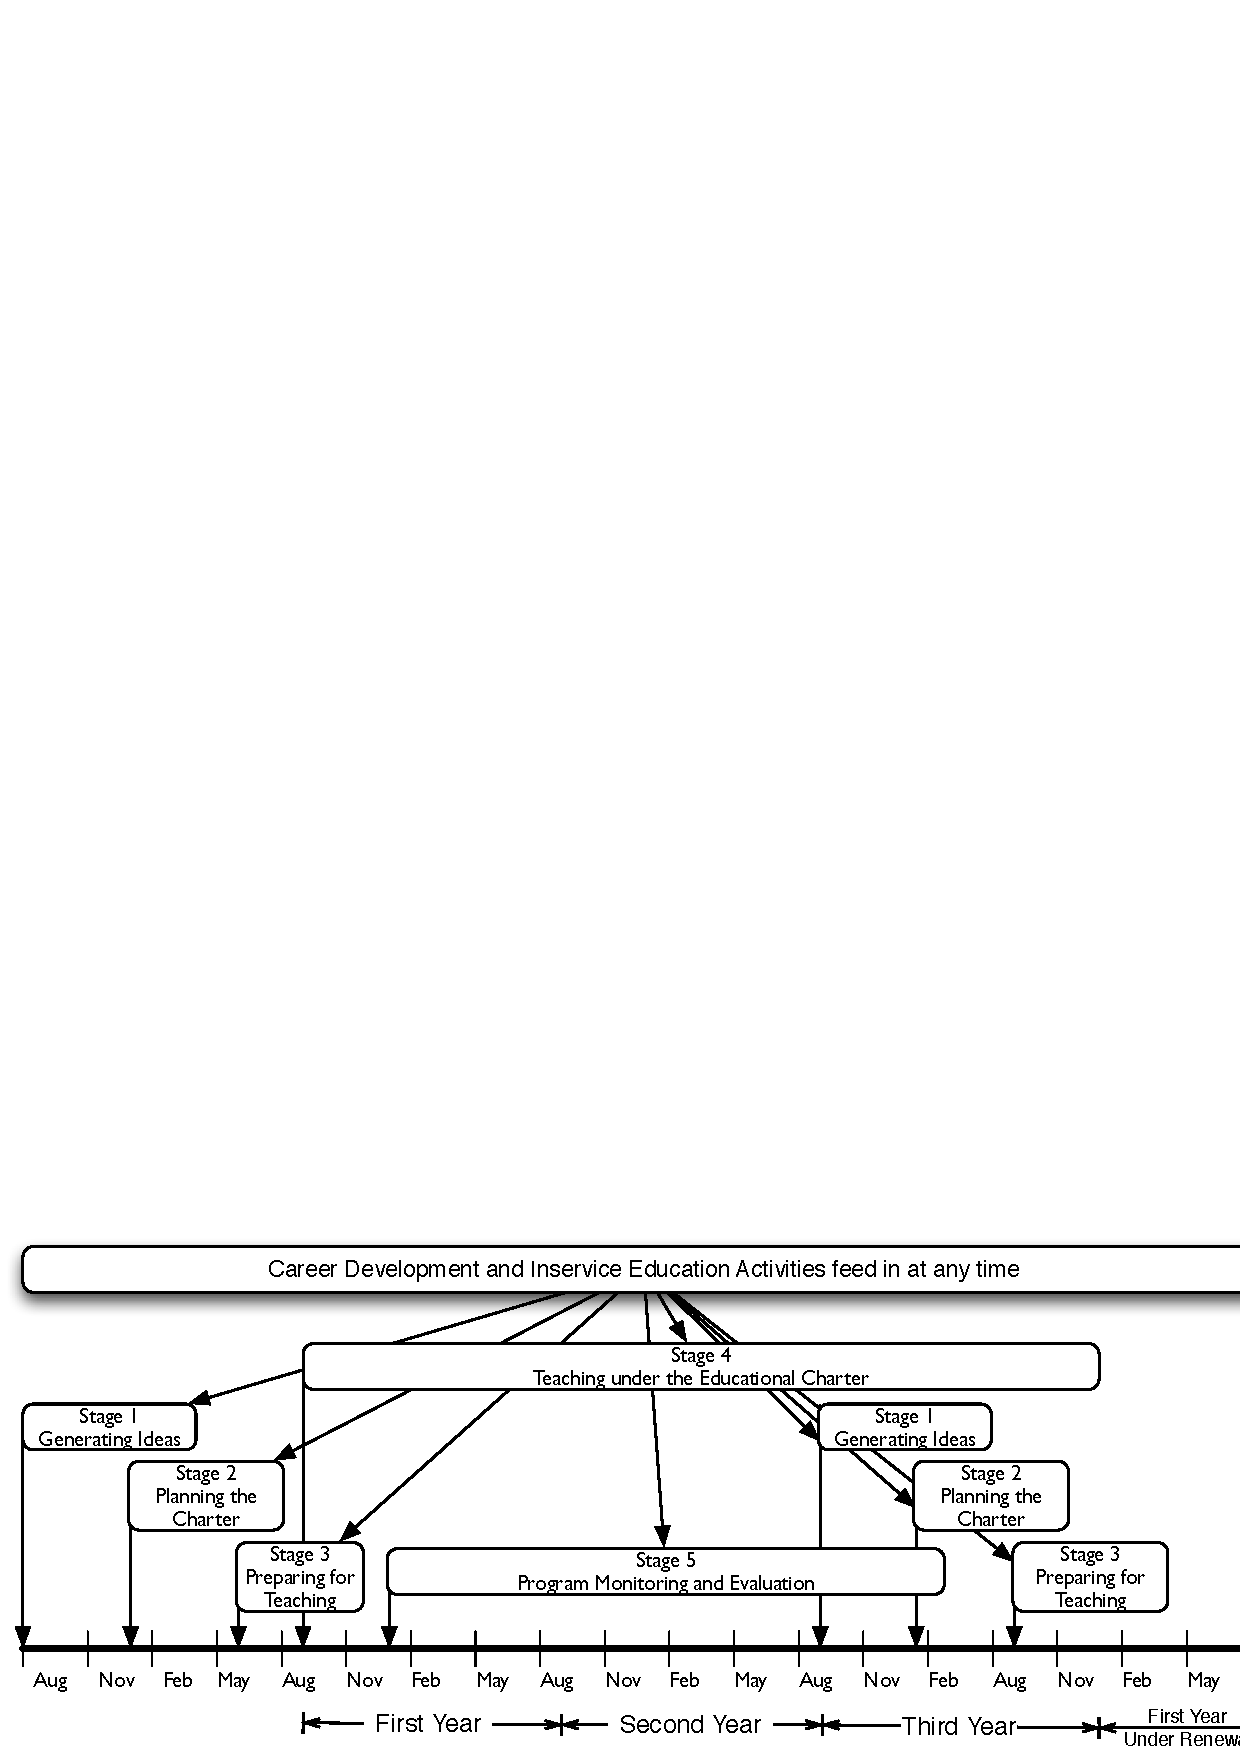
\includegraphics[width=\textwidth]{../Figures/Timeline.pdf}
	
	\small \cite<Adapted from>{Budde1988}
\end{frame}

\begin{frame}[c]
	\frametitle{Growth in Number of Charter Schools}
	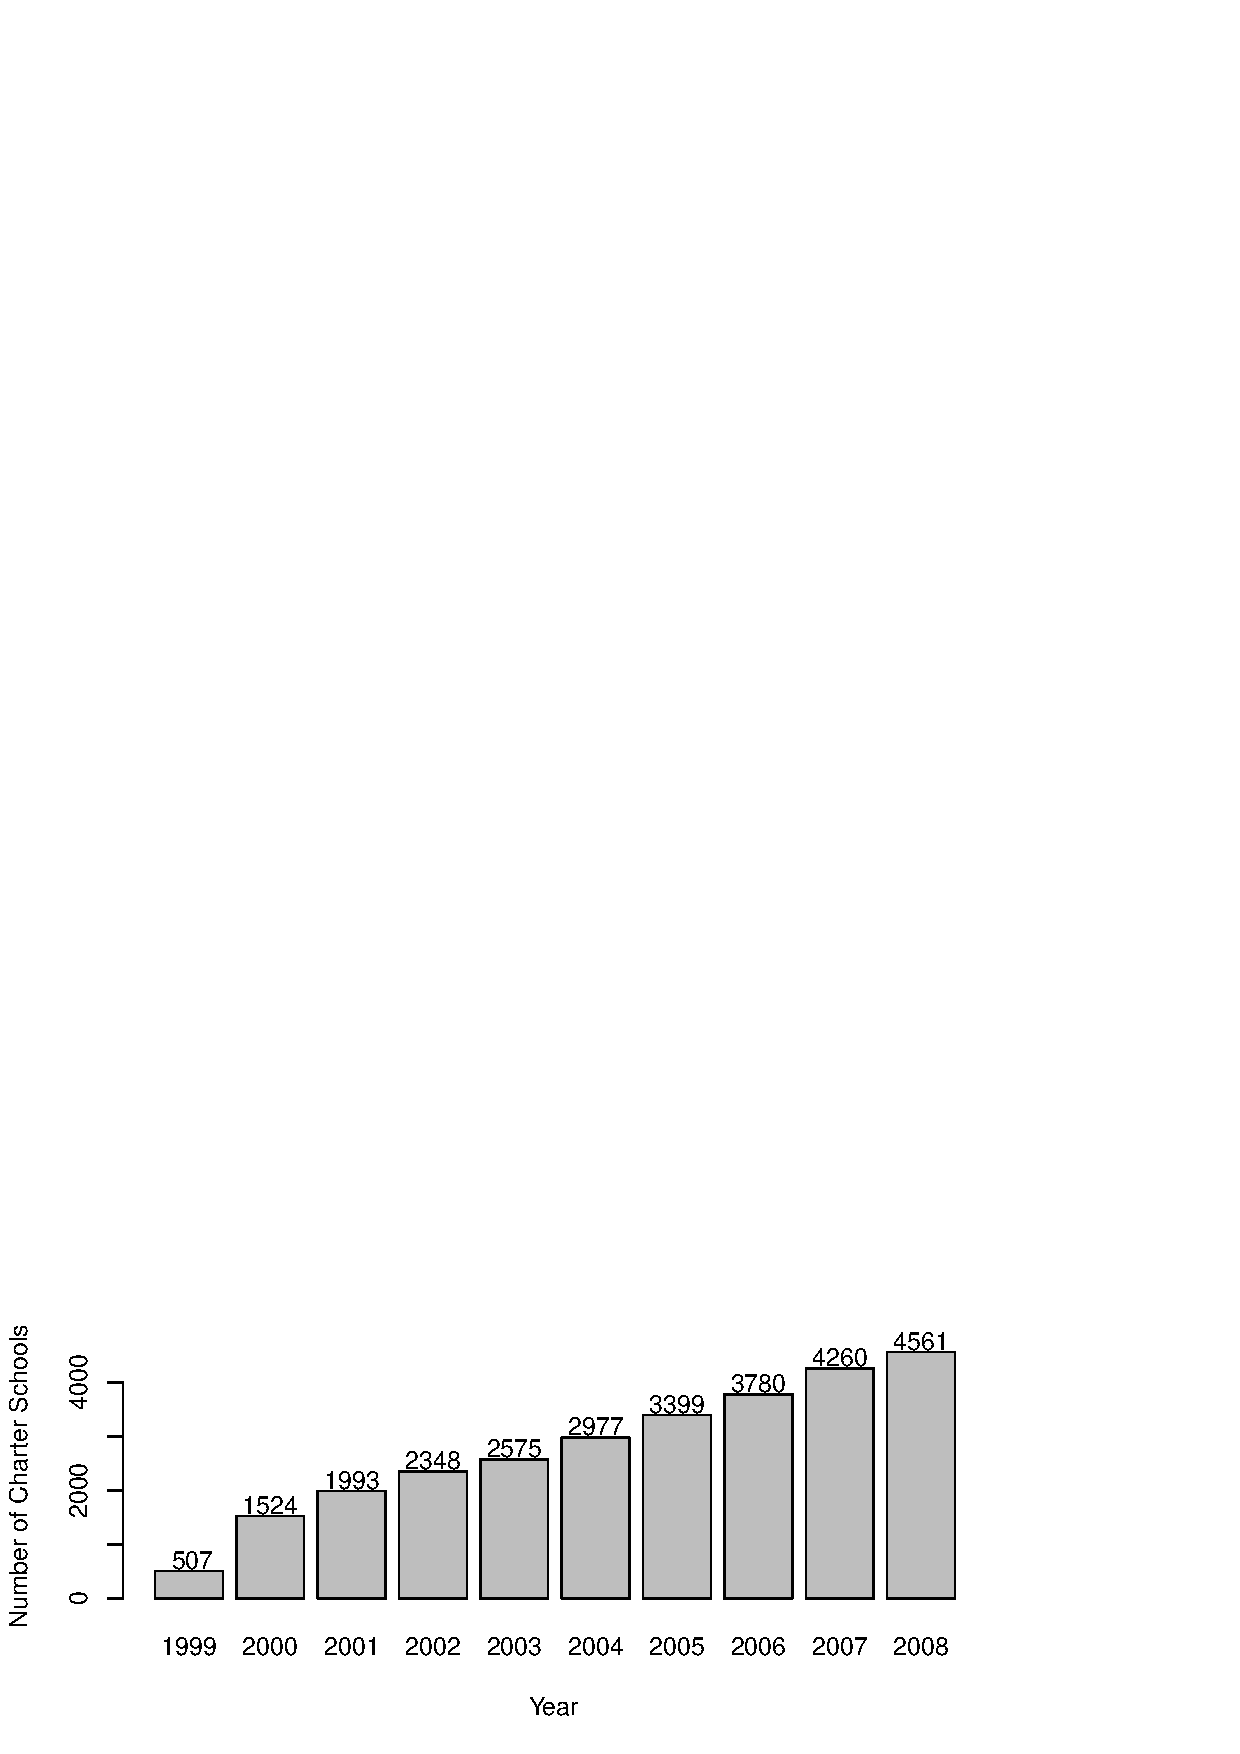
\includegraphics[width=\textwidth]{../Figures/CharterSchoolGrowth.pdf}
\end{frame}

\begin{frame}[c]
	\frametitle{Charter Schools are National (Operating)}
	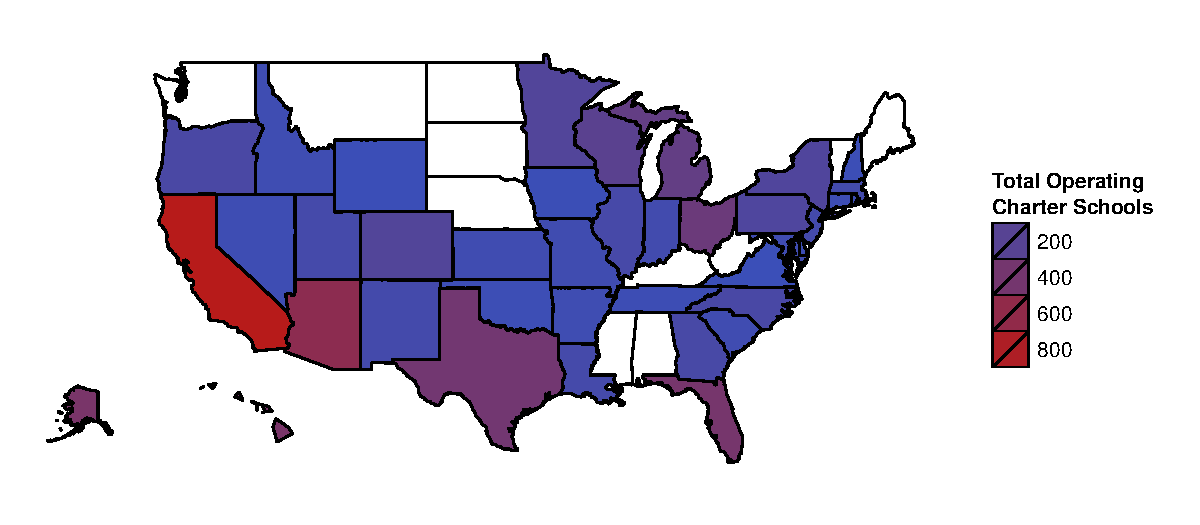
\includegraphics[width=\textwidth]{../Figures/CharterMapOperating.pdf}
\end{frame}

\begin{frame}[c]
	\frametitle{Charter Schools are National (Enrollment)}
	\includegraphics[width=\textwidth]{../Figures/CharterMapEnrollment}
\end{frame}

\begin{frame}[c]
	\frametitle{National Studies Examining Charter and Traditional Public Schools}
	\begin{enumerate}
		\item \citeA{BraunJenkinsGrigg2006} examined charter and traditional public schools using hierarchal linear modeling (HLM) with NAEP 2005. They found that there was often no difference, and in some instances charter school students performed worse.
		\pause
		\item \textit{The CREDO Study} - \citeA{credo} conducted a study of more than 1.7 million records from 2400 charter within 16 states. The methodology involves creating a Virtual Control Record (VCR) for each charter school student which is used to find matching student from an eligible traditional public school.
		Overall results show that charter school students performed, on average, 0.01 and 0.03 standard deviations below public school students for reading and math, respectively.
	\end{enumerate}
\end{frame}

\begin{frame}[c]
\begin{quote}    %Good quote... come back to the idea at some point!
If, however, charter schools are not improving the achievement of disadvantaged children, it may be that the cause of low student performance is not bureaucratic rules but something else. When a treatment is based on a diagnosis, and the treatment doesn't work, it is prudent to examine not only whether the treatment should be improved, but also whether the diagnosis might be flawed. \cite{Carnoy2005}
\end{quote}
\end{frame}

\begin{frame}[c]
	\frametitle{Issues with Charter Schools Research}
	\begin{enumerate}[<+-| alert@+>]
		\item The issue of selection bias
		\item The variation in types or kinds of charter schools.
		\item The nature of student achievement. Research has shown there are numerous factors that contribute to student success including, but not limited to, social economic status, parental education, motivation, etc. The ability to decipher how school choice contributes to student learning in the context of all the other factors cannot help but be difficult.
	\end{enumerate}
\end{frame}

\begin{frame}[c]
	\frametitle{Guiding Research Questions}
	\begin{enumerate}[<+-| alert@+>]
	\item Given appropriate adjustments based on available student data, is there a discernible difference between charter and public schools with regard to math and reading scores at grades 4 and 8?

	\item If so, what is the nature and magnitude of this difference for the two outcomes reading and mathematics (for two grade levels)?
	
	\item And finally, do identified differences differ between states with differing charter school laws? 	
	\end{enumerate}
\end{frame}

\section{Method}

\begin{frame}
	\frametitle{Propensity Score Analysis}
	\begin{enumerate}
		\item \textit{Propensity score analysis using stratification.}
		\begin{enumerate}
			\item Full logistic regression. This method will estimate propensity scores using logistic regression with all available covariates.
			\item Logistic regression with step AIC. The \texttt{stepAIC} in the \texttt{MASS} package \cite{mass} will select the best logistic model based upon the Akaike Information Criterion \cite{Akaike1974}. 
			\item Conditional inference trees.
		\end{enumerate}
	\pause
	\item \textit{Propensity score matching.} 
		\begin{enumerate}
			\item One-to-one
			\item One-to-five
			\item One-to-ten.
		\end{enumerate}
		A dependent sample analysis will be performed on the resulting matched pairs \cite{Austin2011}.
	\pause
	\item \textit{Multilevel propensity score analysis.}
		\begin{enumerate}
			\item Full logistic regression.
			\item Logistic regression with step AIC.
			\item Conditional inference trees.
		\end{enumerate}
	\end{enumerate}
\end{frame}

\begin{frame}[c]
	\frametitle{National Assessment of Educational Progress (NAEP)}
	\begin{enumerate}
	\item Congressionally mandeted.
	\item Started in 1971
	\item Provides national measures of student achievement in many subjects including mathematics, reading, science, writing, history, civics, and the arts. 
	\item The 2007 assessment included over 6,000 public schools and over 200 charter schools comprising of over 145,000 and 3,000 students, respectively. 
	\end{enumerate}
\end{frame}

\begin{frame}
	\frametitle{Covariates Available from NAEP}
	\begin{enumerate}\small{
	\item Are you Hispanic or Latino? [No, I am not Hispanic or Latino; Yes, I am Mexican, Mexican American, or Chicano; Yes, I am Puerto Rican or Puerto Rican American; Yes, I am Cuban or Cuban American; Yes, I am from some other Hispanic or Latino background]
	\item Which of the following best describes you? [White; Black or African American; Asian; American Indian or Alaska Native; Native Hawaiian or other Pacific Islander]
	\item Does your family get a newspaper at least four times a week?
	\item Does your family get any magazines regularly?
	\item About how many books are there in your home?
	\item Is there a computer at home that you use?
	\item Is there an encyclopedia in your home? It could be a set of books, or it could be on the computer.
	\item About how many pages a day do you have to read in school and for homework?
	\item How often do you talk about thinks you have studied in school with someone in your family?
	\item How many days were you absent from school in the last month?
	\item How far in school did your mother go? [Grade 8 Only]
	\item How far in school did your father go? [Grade 8 Only]
	\item How often do people in your home talk to each other in language other than English?
	}
\end{enumerate}
\end{frame}

\begin{frame}[c]
	\frametitle{Missing Data}
	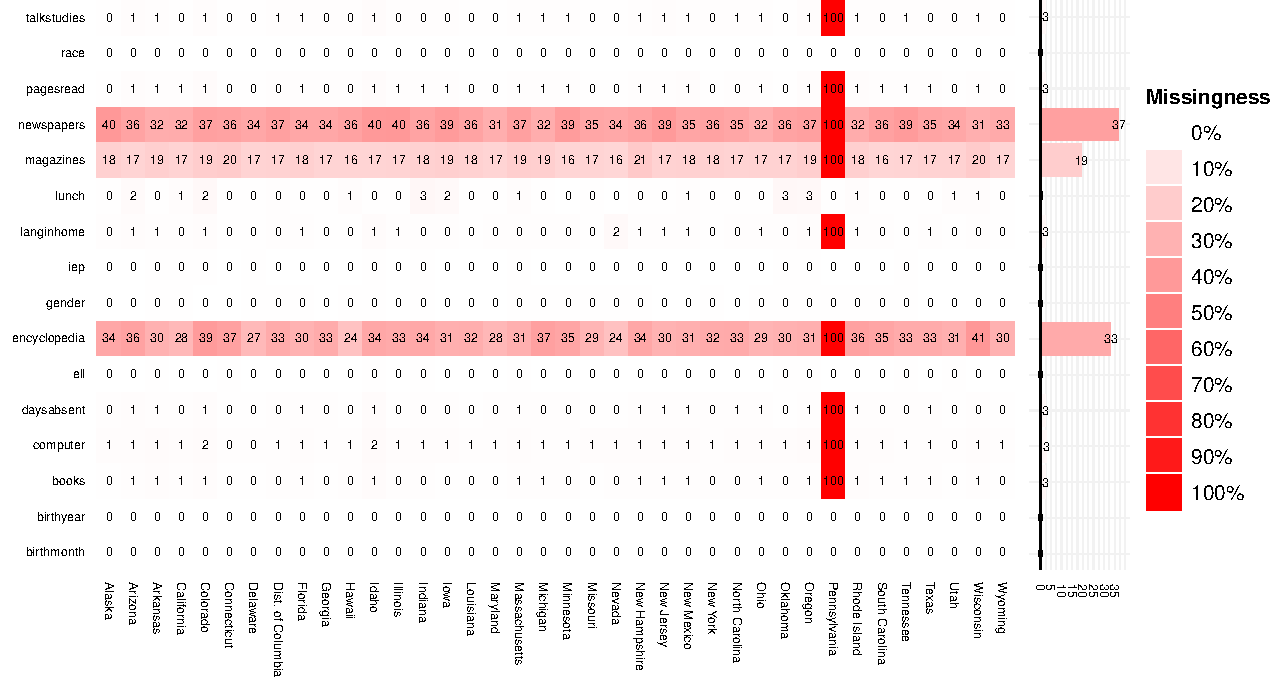
\includegraphics[width=.95\paperwidth]{../Figures/g4mathmissing.pdf} \\
	For the logistic regression models the \texttt{MICE} \cite{Vanbuuren} package will be used to impute missing values.
\end{frame}


\section{Analysis}


{ % Figure that fills the frame
    \setbeamertemplate{navigation symbols}{}
    \begin{frame}[plain]
        \begin{tikzpicture}[remember picture,overlay]
            \node[at=(current page.center)] {
                \includegraphics[heigth=\paperheight]{../Figures/g4mathtreeHeat}
            };
        \end{tikzpicture}
     \end{frame}
}

\subsection{Visualizing Multilevel PSA}
{ % Figure that fills the frame
    \setbeamertemplate{navigation symbols}{}
    \begin{frame}[plain]
        \begin{tikzpicture}[remember picture,overlay]
            \node[at=(current page.center)] {
                \includegraphics[heigth=\paperheight]{../Figures/AnnotatedCircPlot}
            };
        \end{tikzpicture}
     \end{frame}
}

\section{Preliminary Results}

{ % Figure that fills the frame
    \setbeamertemplate{navigation symbols}{}
    \begin{frame}[plain]
        \begin{tikzpicture}[remember picture,overlay]
            \node[at=(current page.center)] {
                \includegraphics[heigth=\paperheight]{../Figures/g4mathlraiccircplot}
            };
        \end{tikzpicture}
     \end{frame}
}

{ % Figure that fills the frame
    \setbeamertemplate{navigation symbols}{}
    \begin{frame}[plain]
        \begin{tikzpicture}[remember picture,overlay]
            \node[at=(current page.center)] {
                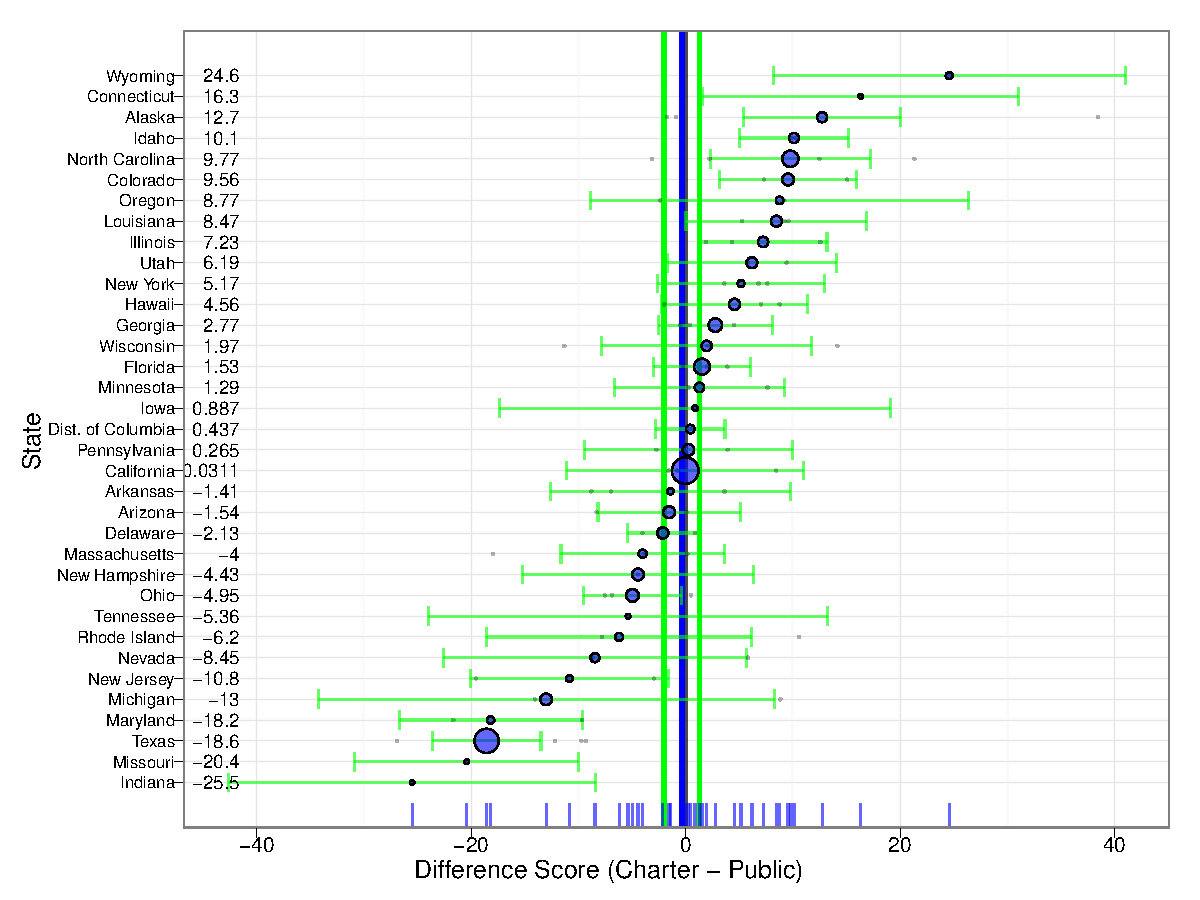
\includegraphics[heigth=\paperheight]{../Figures/g4mathlraicdiffplot}
            };
        \end{tikzpicture}
     \end{frame}
}

{ % Figure that fills the frame
    \setbeamertemplate{navigation symbols}{}
    \begin{frame}[plain]
        \begin{tikzpicture}[remember picture,overlay]
            \node[at=(current page.center)] {
                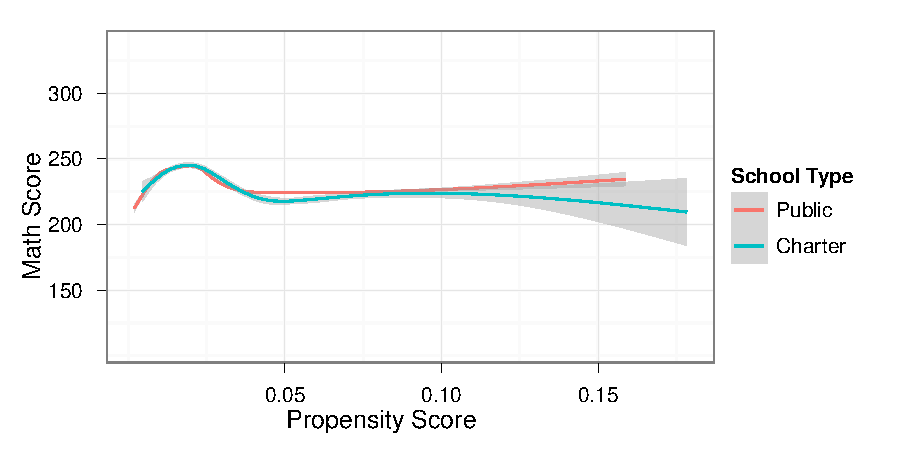
\includegraphics[heigth=\paperheight]{../Figures/g4mathloess}
            };
        \end{tikzpicture}
     \end{frame}
}

{ % Figure that fills the frame
    \setbeamertemplate{navigation symbols}{}
    \begin{frame}[plain]
        \begin{tikzpicture}[remember picture,overlay]
            \node[at=(current page.center)] {
                \includegraphics[heigth=\paperheight]{../Figures/overallsummary}
            };
        \end{tikzpicture}
     \end{frame}
}


\section{Discussion}

\begin{frame}[c]
	\frametitle{Related Projects}
	\begin{itemize}
		\item All of the R and \LaTeX{} code will be available on Github (\url{http://github.com/jbryer/Dissertation}).
		\item \texttt{multilevelPSA} - An R package for the methods outlined here. Hosted at \url{http://github.com/jbryer/multilevelPSA}
		\item \texttt{naepR} - An R package for accessing and analyzing NAEP data. This work is being supported by Educational Testing Services.
		\item I am writing a chapter on using NAEP with R for the \textit{NAEP Primer} with Emmanual Sikali.
	\end{itemize}
\end{frame}


\begin{frame}[c]
	\LARGE{Thank You}\\
	\normalsize
	\ \\
	Jason Bryer (jason@bryer.org)\\
	\ \\
	\url{http://bryer.org}\\
	\url{http://github.com/jbryer/Dissertation}\\
	\url{http://github.com/jbryer/multilevelpsa}
\end{frame}

\begin{frame}[c,shrink=30]
	\frametitle{References}
	\bibliographystyle{apacite}
	\bibliography{Bibliography}
\end{frame}


\end{document}
